\section{Question 1- Nodal Analysis}


\subsection{Theoretical Analysis}




\subsection{Operating Point Analysis}
First of all, to contextualize the values obtained using the tools in ngspice, it is necessary to state that, as node 0 is connected to ground, its nodal voltage does not appear on the table of results. Furthermore, to be able to describe the voltage flowing in the dependent source, it is necessary to know the current in resistor 6. However, ngspice is not able to compute this value when the depedent source is described. So, in order to do that, an extra dependent voltage source (whose voltage drop is equal to 0 V) was created, and put in series after the resistor 6. This led to the appearence of node 8, that has the same voltage drop as node 6. So, by doing that, ngspice is able to determine the current in this auxiliar independent source, which is exactly the value needed.
 The circuit with these changes is shown in the drawing below.

\begin{figure}[ht] \centering
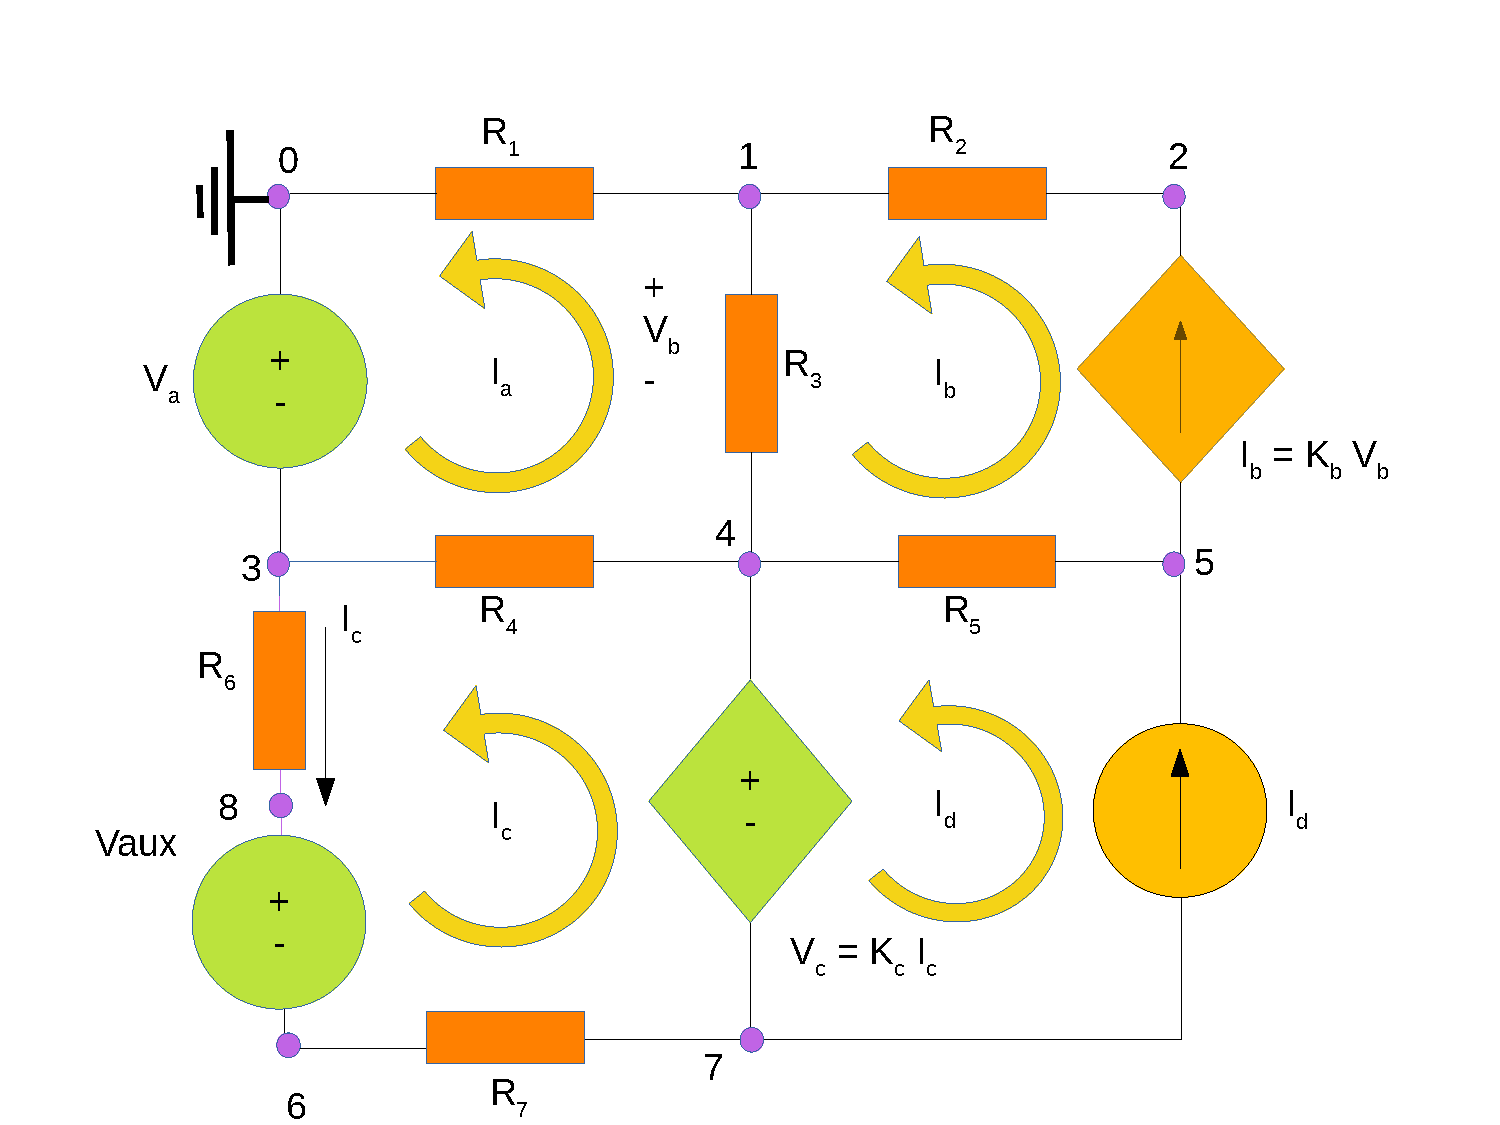
\includegraphics[width=1.0\linewidth]{simdraw.pdf}
\caption{Circuit analysed in ngspice.}
\label{simdraw}
\end{figure}

\subsection{Comparison}
After running the simulation, the results were put in the table below. Then, a careful analysis of the aforementioned table was conducted.It shows the simulated operating point results for the circuit that is being studied, allowing the group to obtain the current flowing in every risistor, the voltage in the dependent voltage source and even the current flowing in the dependent currrent source. 

A variable preceded by @ is of type {\em current} and expressed in Ampere; other variables are of type {\it voltage} and expressed in
    Volt.
\begin{table}[ht]
\parbox{.45\linewidth}{
  \centering
  \begin{tabular}{|l|r|}
    \hline    
    {\bf Name} & {\bf Value [A or V]} \\ \hline
    @c1[i] & 0.000000e+00\\ \hline
@gb[i] & -2.26065e-04\\ \hline
@r1[i] & 2.161572e-04\\ \hline
@r2[i] & -2.26065e-04\\ \hline
@r3[i] & -9.90741e-06\\ \hline
@r4[i] & 1.183330e-03\\ \hline
@r5[i] & -2.26065e-04\\ \hline
@r6[i] & -9.67173e-04\\ \hline
@r7[i] & 9.671730e-04\\ \hline
v(1) & 5.068716e+00\\ \hline
v(2) & 4.843672e+00\\ \hline
v(3) & 4.369060e+00\\ \hline
v(5) & 4.874693e+00\\ \hline
v(6) & 5.579017e+00\\ \hline
v(7) & -1.98076e+00\\ \hline
v(8) & -2.97458e+00\\ \hline
v(9) & -1.98076e+00\\ \hline

  \end{tabular}
  \caption{Simulation and Calculus of Req (NgSpice)}}
 
\parbox{.45\linewidth}{
  \centering
  \begin{tabular}{|l|r|}
    \hline    
    {\bf Name} & {\bf Value [A or V]} \\ \hline
    V1 & 5.068716e+00 \\ \hline
V2 & 4.843672e+00 \\ \hline
V3 & 4.369060e+00 \\ \hline
V4 & 0.000000e+00 \\ \hline
V5 & 4.874693e+00 \\ \hline
V6 & 5.579017e+00 \\ \hline
V7 & -1.980764e+00 \\ \hline
V8 & -2.974577e+00 \\ \hline

  \end{tabular}
  \caption{Simulation and Calculus of Req (NgSpice)}}
 
\end{table}


In order to validate the results obtained in NGSPICE, relative errors between the theoretical values, obtained in octave and the ones obtained in ngspice, were calculated. These were put in the table below.

\begin{table}[ht] \centering
\begin{tabular}{|
>{\columncolor[HTML]{FFCC67}}l |c|}
\hline
\multicolumn{2}{|l|}{\cellcolor[HTML]{EABD8B}Relative Errors (\%)} \\ \hline
{\color[HTML]{333333} V1}               & 4.444e-05               \\ \hline
{\color[HTML]{333333} V2}               & 4.288e-05               \\ \hline
{\color[HTML]{333333} V3}               & 7.892e-05               \\ \hline
{\color[HTML]{333333} V4}               & 5.154e-05               \\ \hline
{\color[HTML]{333333} V5}               & 0                       \\ \hline
{\color[HTML]{333333} V6}               & 0                       \\ \hline
{\color[HTML]{333333} V7}               & 2.487e-05               \\ \hline
{\color[HTML]{333333} IA}               & 9.253e-05               \\ \hline
{\color[HTML]{333333} IB}               & 1.769e-05               \\ \hline
{\color[HTML]{333333} IC}               & 0                       \\ \hline
\end{tabular}
\caption{Relative Errors between Octave and NgSpice results}
\end{table}




After the anaylysis of these errors, we conclude that the accuracy is extremely high supported by the fact that the relative maximum error is 9.253e-05\%. Nevertheless, we assume that these errors are due to dissipated power in the resistors. Even so, the simulation results can be validated.

